\documentclass[12pt, a4paper, simple]{eskdtext}

\usepackage{hyperref}
\usepackage{env}
\usepackage{_sty/gpi_lst}
\usepackage{_sty/gpi_toc}
\usepackage{_sty/gpi_t}
\usepackage{_sty/gpi_p}

\def \gpiPrilLetter {A}

% Код
\ESKDletter{}{К}{П}
\def \gpiDocTypeNum {90}
\def \gpiCode {\ESKDtheLetterI\ESKDtheLetterII\ESKDtheLetterIII.\gpiStudentGroupName\gpiStudentGroupNum.\gpiStudentCard~-~0\gpiDocNum~\gpiDocTypeNum~\gpiDocVersion}

\def \gpiDocTopic {НАБОР ТЕСТОВЫХ ЗАДАНИЙ ДЛЯ ПРОВЕРКИ}

% колонтитулы
\usepackage{fancybox, fancyhdr}
\fancypagestyle{plain}
{
    \renewcommand{\footrulewidth}{0pt}          % Толщина отделяющей полоски снизу
    \renewcommand{\headrulewidth}{0pt}          % Толщина отделяющей полоски сверху
    \fancyhead[C]{\hfill\gpiCode\hfill\thepage} % Сверху по центру выводить код
    \fancyfoot{}                                % Очистить нижний колонтитул
}

% Графа 1 (наименование изделия/документа)
\ESKDcolumnI {\ESKDfontII \gpiTopic \\ \gpiDocTopic}

% Графа 2 (обозначение документа)
\ESKDsignature {\gpiCode}

% Графа 9 (наименование или различительный индекс предприятия) задает команда
\ESKDcolumnIX {\gpiDepartment}

% Графа 11 (фамилии лиц, подписывающих документ) задают команды
\ESKDcolumnXIfI {\gpiStudentSurname}
\ESKDcolumnXIfII {\gpiTeacherSurname}
\ESKDcolumnXIfV {\gpiTeacherSurname}

\renewcommand {\thefigure} {\arabic{figure}}

\begin{document}
    \begin{ESKDtitlePage}
    \begin{flushright}
        \textbf{ПРИЛОЖЕНИЕ \gpiPrilLetter} \enspace\enspace
    \end{flushright}
    \begin{center}
        % \gpiMinEdu \\
        \gpiEdu \\
        \gpiKaf \\
    \end{center}

    \vfill

    \begin{center}
        \gpiTopic \\
    \end{center}

    \vfill

    \begin{center}
        \textbf{\gpiDocTopic} \\
    \end{center}

    \vfill

    \begin{center}
        \gpiCode \\
        Листов \pageref{LastPage} \\
    \end{center}

    \vfill

    \begin{flushright}
        \begin{minipage}[t]{.49\textwidth}
            \begin{minipage}[t]{.75\textwidth}
                \begin{flushright}
                    Руководитель

                    Выполнил

                    Консультант

                    по ЕСПД
                \end{flushright}
            \end{minipage}
        \end{minipage}
        \begin{minipage}[t]{.49\textwidth}
            \begin{flushright}
                \begin{minipage}[t]{.75\textwidth}
                    \gpiTeacherName~\gpiTeacherSurname

                    \gpiStudentName~\gpiStudentSurname

                    \hspace{0pt}

                    \gpiTeacherName~\gpiTeacherSurname

                \end{minipage}
            \end{flushright}
            
        \end{minipage}
    \end{flushright}

    \vfill

    \begin{center}
        \ESKDtheYear
    \end{center}
\end{ESKDtitlePage}


    \ESKDstyle{title}
    \thispagestyle{plain}
    \pagestyle{plain}
    \hspace{0pt}

    В данном приложении приведены эталоны документов,
    являющиеся тестовым набором данных для проверки разработанной базы данных.

    На рисунке~\ref{fig:CP_MoiOrg_etalon} представлен эталон справочного документа <<Мои организации>>.

    На рисунке~\ref{fig:CP_EdHran_etalon} представлен эталон справочного документа <<Единицы хранения>>.

    \begin{figure}[!h]
        \centering
        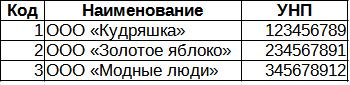
\includegraphics[]
            {_docs/СП_МоиОрг_эталон.jpg}
        \caption{Эталон справочника <<Мои организации>>}
        \label{fig:CP_MoiOrg_etalon}
    \end{figure}

    \begin{figure}[!h]
        \centering
        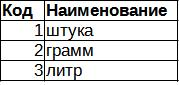
\includegraphics[]
            {_docs/СП_ЕдХран_эталон.jpg}
        \caption{Эталон справочника <<Единицы хранения>>}
        \label{fig:CP_EdHran_etalon}
    \end{figure}

\end{document}
